% --- LaTeX Presentation Template - S. Venkatraman ---

% --- Set document class ---

% Remove "handout" when presenting to include pauses
\documentclass[dvipsnames, handout]{beamer}


\usepackage{algorithm}
\usepackage{algpseudocode}
\usepackage[square,numbers]{natbib}

\usetheme{default}

% Make content that is hidden by pauses "transparent"
\setbeamercovered{transparent}

% --- Slide layout settings ---

% Set line spacing
\renewcommand{\baselinestretch}{1.15}

% Set left and right text margins
\setbeamersize{text margin left=12mm, text margin right=12mm}

% Add slide numbers in bottom right corner
\setbeamertemplate{footline}[frame number]

% Remove navigation symbols
\setbeamertemplate{navigation symbols}{}

% Allow local line spacing changes
\usepackage{setspace}

% Change itemized list bullets to circles
\setbeamertemplate{itemize item}{$\bullet$}
\setbeamertemplate{itemize subitem}{$\circ$}

% --- Color and font settings ---

\usepackage{xcolor}


% Slide title background color
\definecolor{background}{HTML}{ede6d8}

% Slide title text color
\definecolor{titleText}{HTML}{B40404}

% Other possible color schemes

% - Light green/dark green -
%\definecolor{background}{HTML}{e4ede4}
%\definecolor{titleText}{HTML}{2e592f}

% - Light blue/dark blue -
%\definecolor{background}{HTML}{d5d9e8}
%\definecolor{titleText}{HTML}{2d375e}

% - Beige/dark blue -
%\definecolor{background}{HTML}{e8e2d5}
%\definecolor{titleText}{HTML}{2d3375}

% Set colors
\setbeamercolor{frametitle}{bg=background, fg=titleText}
\setbeamercolor{subtitle}{fg=titleText}

% Set font sizes for frame title and subtitle
\setbeamerfont{frametitle}{size=\fontsize{15}{16}}
\setbeamerfont{framesubtitle}{size=\small}

% --- Math/Statistics commands ---

% Add a reference number to a single line of a multi-line equation
% Usage: "\numberthis\label{labelNameHere}" in an align or gather environment
\newcommand\numberthis{\addtocounter{equation}{1}\tag{\theequation}}

% Shortcut for bold text in math mode, e.g. $\b{X}$
\let\b\mathbf

% Shortcut for bold Greek letters, e.g. $\bg{\beta}$
\let\bg\boldsymbol

% Shortcut for calligraphic script, e.g. %\mc{M}$
\let\mc\mathcal

% \mathscr{(letter here)} is sometimes used to denote vector spaces
\usepackage[mathscr]{euscript}

% Convergence: right arrow with optional text on top
% E.g. $\converge[p]$ for converges in probability
\newcommand{\converge}[1][]{\xrightarrow{#1}}

% Weak convergence: harpoon symbol with optional text on top
% E.g. $\wconverge[n\to\infty]$
\newcommand{\wconverge}[1][]{\stackrel{#1}{\rightharpoonup}}

% Equality: equals sign with optional text on top
% E.g. $X \equals[d] Y$ for equality in distribution
\newcommand{\equals}[1][]{\stackrel{\smash{#1}}{=}}

% Normal distribution: arguments are the mean and variance
% E.g. $\normal{\mu}{\sigma}$
\newcommand{\normal}[2]{\mathcal{N}\left(#1,#2\right)}

% Uniform distribution: arguments are the left and right endpoints
% E.g. $\unif{0}{1}$
\newcommand{\unif}[2]{\text{Uniform}(#1,#2)}

% Independent and identically distributed random variables
% E.g. $ X_1,...,X_n \iid \normal{0}{1}$
\newcommand{\iid}{\stackrel{\smash{\text{iid}}}{\sim}}

% Sequences (this shortcut is mostly to reduce finger strain for small hands)
% E.g. to write $\{A_n\}_{n\geq 1}$, do $\bk{A_n}{n\geq 1}$
\newcommand{\bk}[2]{\{#1\}_{#2}}

% Math mode symbols for common sets and spaces. Example usage: $\R$
\newcommand{\R}{\mathbb{R}}	% Real numbers
\newcommand{\C}{\mathbb{C}}	% Complex numbers
\newcommand{\Q}{\mathbb{Q}}	% Rational numbers
\newcommand{\Z}{\mathbb{Z}}	% Integers
\newcommand{\N}{\mathbb{N}}	% Natural numbers
\newcommand{\F}{\mathcal{F}}	% Calligraphic F for a sigma algebra
\newcommand{\El}{\mathcal{L}}	% Calligraphic L, e.g. for L^p spaces

% Math mode symbols for probability
\newcommand{\pr}{\mathbb{P}}	% Probability measure
\newcommand{\E}{\mathbb{E}}	% Expectation, e.g. $\E(X)$
\newcommand{\var}{\text{Var}}	% Variance, e.g. $\var(X)$
\newcommand{\cov}{\text{Cov}}	% Covariance, e.g. $\cov(X,Y)$
\newcommand{\corr}{\text{Corr}}	% Correlation, e.g. $\corr(X,Y)$
\newcommand{\B}{\mathcal{B}}	% Borel sigma-algebra

% Other miscellaneous symbols
\newcommand{\tth}{\text{th}}	% Non-italicized 'th', e.g. $n^\tth$
\newcommand{\Oh}{\mathcal{O}}	% Big-O notation, e.g. $\O(n)$
\newcommand{\1}{\mathds{1}}	% Indicator function, e.g. $\1_A$

% Additional commands for math mode
\DeclareMathOperator*{\argmax}{argmax}	% Argmax, e.g. $\argmax_{x\in[0,1]} f(x)$
\DeclareMathOperator*{\argmin}{argmin}	% Argmin, e.g. $\argmin_{x\in[0,1]} f(x)$
\DeclareMathOperator*{\spann}{Span}	% Span, e.g. $\spann\{X_1,...,X_n\}$
\DeclareMathOperator*{\bias}{Bias}	% Bias, e.g. $\bias(\hat\theta)$
\DeclareMathOperator*{\ran}{ran}		% Range of an operator, e.g. $\ran(T)
\DeclareMathOperator*{\dv}{d\!}		% Non-italicized 'with respect to', e.g. $\int f(x) \dv x$
\DeclareMathOperator*{\diag}{diag}	% Diagonal of a matrix, e.g. $\diag(M)$
\DeclareMathOperator*{\trace}{trace}	% Trace of a matrix, e.g. $\trace(M)$
\DeclareMathOperator*{\supp}{supp}	% Support of a function, e.g., $\supp(f)$

% --- Presentation begins here ---

\begin{document}

% --- Title slide ---

\title{\color{titleText} Hidden Markov models and sequential Monte Carlo Project :}
\subtitle{\color{Blue} Estimating behavioral parameters in animal
movement models using a state-augmented
particle filter}
\author{B. Maurel - G. Watkinson - J.Stym-Popper - G. Guaquière \vspace{-.3cm}}
\institute{ENSAE Paris}
\date{}

\begin{frame}
\titlepage
\vspace{-1.2cm}
\begin{center}
\includegraphics[width=2.3cm]{logo-ensae.png}\bigskip
\end{center}
\end{frame}

% --- Main content ---

% Example slide: use \pause to sequentially unveil content
\begin{frame}{Introduction}
\framesubtitle{Presentation of the problem}

\citet{dowd2011estimating} proposed a methodology to model the behavior of seals in their natural habitat, using their vertical velocity.
\newline
\\
Indeed, depth measurements vary depending on whether the seals are hunting, exploring, moving, and so on ...
\newline
\\
They model the animal's behavior with state-space models and estimate the latent behavioral parameters with an algorithm.



% Dowd and Joy proposed a model to gain a deeper understanding of the behavior of seals in their natural habitat, using data on their vertical velocity.
% \newline
% \\
% Depth measurements vary depending on whether the seals are hunting, exploring, moving, and so on.
% \newline
% \\
% To do so, they model the animal's behavior with state-space models using high resolution time series data.

\end{frame}

\begin{frame}{Introduction}
\framesubtitle{Data used}

\begin{figure}
    \centering
    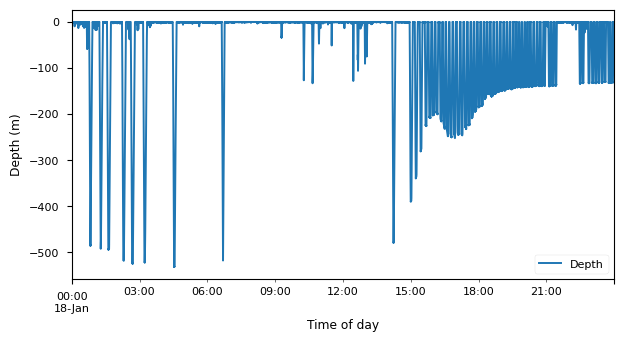
\includegraphics[width=\linewidth]{depth_fig.png}
    \caption{Evolution of the depth (in m) of the seal on January 18th, 2008, taken at 5 second intervals.}
    \label{fig:depth}
\end{figure}
\end{frame}

\begin{frame}{Introduction}
\framesubtitle{Data used}
\begin{figure}
    \centering
    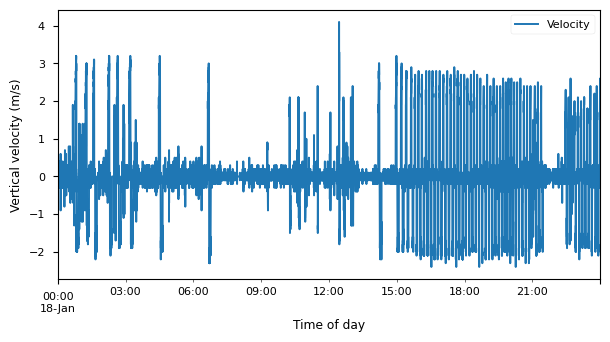
\includegraphics[width=\linewidth]{velocity_fig.png}
    \caption{Vertical velocity (m/s) of a single seal on January 18th, 2008.}
    \label{fig:velocity}
\end{figure}

\end{frame}

\begin{frame}{First equations}
\framesubtitle{State evolution equation}

We use the following state evolution equation to model a stochastic animal movement :

\begin{equation}
\mathbf{x}_t=\mathbf{f}(\mathbf{x}_{t-1},\mathbf{\theta}_t)+\mathbf{n}_t
\end{equation}

where :
\newline
\\

$\mathbf{x}_t$ = vertical velocity

$\theta_t$ = latent behavioral parameters

$\mathbf{f}$ = the movement

$\mathbf{n}_t$ = system noise.

\end{frame}


\begin{frame}{First equations}
\framesubtitle{Observation equation}
Equation (1) is not ideal because we would prefer the sought-after value $\theta_t$ to follow a Markov process, rather than the observed value $\mathbf{x}_t$
\newline
\\
We artificially augment the state space by introducing the variable $X_t = \begin{pmatrix}
\mathbf{x}_t\\\theta_t
\end{pmatrix}$.
\newline
\\
The observation equation is given by $y_t = HX_t + e_t$, where $H = (1, 0)$
\newline
\\
$y_t$ represents the observation of vertical velocity at time $t$

$e_t$, the observation error, is a normal noise term.

\end{frame}

\begin{frame}{First equations}
\framesubtitle{Markov process}

We seek a Markov process of the form:
\begin{equation}
\begin{pmatrix}
\mathbf{x}_t\\\theta_t
\end{pmatrix}
=
\mathbf{f}\begin{pmatrix}
\mathbf{x}_{t-1}\\\theta_{t-1}
\end{pmatrix}
+
\begin{pmatrix}
\mathbf{n}_t \\\mathbf{v}_t
\end{pmatrix}
\end{equation}

\end{frame}

\begin{frame}{First equations}
\framesubtitle{How to deal with $\theta_{t}$}

Problem : there is no consistent model to represent the evolution of $\theta_{t}$
\newline
\\
Since it represents the behavioral the seal, this parameters is constant over by period.
We consider windows of 26 minutes and we make the assumption that $\theta_{t}$ is constant over each window.
\newline
\\
To estimate $\theta_{t}$, we still introduce an arbitrary movement on $\theta_{t}$:
\begin{center}

$\theta_t = \theta_{t-1} + \nu_t$

\end{center}
where $v_t$ follows a normal distribution with variance $\sigma_\nu^2$.\\

\end{frame}

\begin{frame}{First equations}
\framesubtitle{Definition of the movement model f}

$f$ characterizes the movement of the seal
\newline
\\
We use an $AR(2)$ to describe the vertical velocity of a seal :
\begin{equation}
z_t = a_1z_{t-1} + a_2z_{t-2} + \epsilon_t
\end{equation}

In order to have a Markov process, we augmented the state space with the dummy variable $\zeta_t$, such that:
\begin{equation}
\begin{pmatrix}
\mathbf{z}_t\\\mathbf{\zeta}_t
\end{pmatrix}
=
\begin{pmatrix}
a_{1,t}& a_{2,t} \\
1 & 0
\end{pmatrix}
\begin{pmatrix}
\mathbf{z}_{t-1}\\\mathbf{\zeta}_{t-1}
\end{pmatrix}
+
\begin{pmatrix}
\mathbf{\epsilon}_t \\ 0
\end{pmatrix}
\end{equation}
\end{frame}

\begin{frame}{Final form}
\framesubtitle{Movement model}

Taking into account both state augmentations, we end up with the movement model :
\begin{equation}
\label{eqn:markov process}
    \mathbf{X_t} =
    \begin{pmatrix}
    \mathbf{z_t}\\\mathbf{\zeta_t}\\ a_{1,t}\\ a_{2,t}
    \end{pmatrix}
    =
    \begin{pmatrix}
    a_{1,t-1}& a_{2,t-1} & 0 & 0\\
    1 & 0 & 0 & 0\\
    0 & 0 & 1 & 0\\
    0 & 0 & 0 & 1\\

    \end{pmatrix}
    \begin{pmatrix}
    \mathbf{z}_{t-1}\\\mathbf{\zeta}_{t-1}\\ a_{1, t-1} \\ a_{2,t-1}
    \end{pmatrix}
    +
    \begin{pmatrix}
    \mathbf{\varepsilon}_t \\ 0 \\ \nu_{1,t} \\\nu_{2,t}
    \end{pmatrix}
\end{equation}

 The system noise $\varepsilon_t$ takes the form of a normal mixture process that allows for occasional large values, $\varepsilon_t \sim 0.9 \mathcal{N}({0},{\sigma_{\varepsilon}^2}) + 0.1 \mathcal{N}({0},{10\sigma_{\varepsilon}^2})$.
 \newline
\\
 Meanwhile, $\nu_{1,t}$ and $\nu_{2,t}$ are random noise for the random walk of the parameters, $\nu_{1,t}, \nu_{2,t} \sim \mathcal{N}({0},{\sigma_{\nu}^2})$.
\end{frame}

\begin{frame}{Final form}
\framesubtitle{Movement model}

And the observation model :

\begin{equation}
\label{eqn:y sachant X}
    \mathbf{y}_t =
    \begin{pmatrix}
    1 & 0 & 0 & 0
    \end{pmatrix}
    \begin{pmatrix}
        \mathbf{z_t}\\\mathbf{\zeta_t}\\a_{1,t}\\ a_{2,t}
    \end{pmatrix}
    +
    \mathbf{e_t}
\end{equation}
with the observation error $\mathbf{e_t} \sim \mathcal{N}(0,{\sigma_{o}^2})$. It can be rewritten as $\mathbf{y}_t = G_t \mathbf{X_t} + \mathbf{e_t}$.

This leads to the associated Feynman-Kac model where :
\begin{itemize}
    \item $M_t$ is the Hidden Markov Process described in (Eq. \ref{eqn:markov process}).
    \item $G_t$ is the density of $\mathbf{y_t}$ knowing $\mathbf{X_t}$ (Eq. \ref{eqn:y sachant X}).
\end{itemize}

\end{frame}

\begin{frame}{The algorithm of the paper}
\framesubtitle{Estimation of $\theta= \begin{pmatrix}
    a_{1}\\ a_{2}
\end{pmatrix}$\ inside a time window}

\begin{algorithmic}[1]
% \Require A time window $w_i = [y_1, \dots ,y_T]$
% \Ensure An estimation of $\theta_i$ on the window
\State $m \gets 0$ \Comment{The iteration step}
\State $\sigma_v^2(0) \gets 0.1$ \Comment{The parameter noise variance}
\State $\theta_0(0) \gets 0$ \Comment{The initial value of the parameter}
\While{$m < 10$}
\State Estimate $\theta_{1,\dots,T}(m)$ using a Particle Filter
\State Update $\theta_0(m+1) \gets \frac{1}{T}\sum_{t = 1}^{T}\theta_t^m$
\State Update $\sigma_v^2(m+1) \gets \alpha\times\sigma_v^2(m)$
\EndWhile
\State Use $\theta_0(10)$ as the estimation for $\theta_i$
\end{algorithmic}

\end{frame}

\begin{frame}{Results using the aglorithm of the paper}
\framesubtitle{Results of 20 run of the aglorithm to estimate $a_1$ and $a_2$}

\begin{figure}
\centering
    \centering
    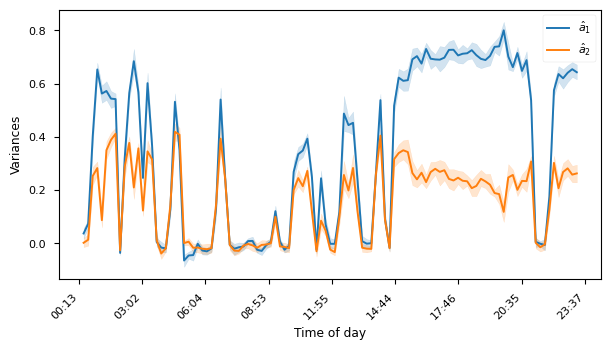
\includegraphics[width=\linewidth]{a1_a2_var_0.5.png}
    \caption{We thus want latent parameters estimate, that translates those states in a mathematical representation easier to analyze at scale.}
    \label{fig:paper_results}
\end{figure}

\end{frame}

\begin{frame}{How to use SMC$^2$ within this context}
\framesubtitle{Definition of the Markov-process}

In that section, we do not assume anymore that $a_1, a_2$ follows a random walk on each window. They are now supposed constant.
\newline
\\
The Markov process used to define the Feynman-Kac model becomes the following:
\begin{equation}
    \mathbf{X_t} =
    \begin{pmatrix}
    \mathbf{z_t}\\\mathbf{\zeta_t}
    \end{pmatrix}
    =
    \begin{pmatrix}
    a_1& a_2\\
    1 & 0

    \end{pmatrix}
    \begin{pmatrix}
    \mathbf{z}_{t-1}\\\mathbf{\zeta}_{t-1}
    \end{pmatrix}
    +
    \begin{pmatrix}
    \mathbf{\epsilon}_t \\ 0
    \end{pmatrix}
\end{equation}

\end{frame}

\begin{frame}{How to use SMC$^2$ within this context}
\framesubtitle{Distribution of interest}

A SMC defined with this Hidden Markov Process will return an estimation of for all $t, \mathbb{P}^{a_1,a_2}(y_{0:T})$.
\newline
\\
To be able to have a good approximation of  of the latent parameters $a_1, a_2$, we would like to estimate the density function:
$$
(a_1, a_2) \xrightarrow{} \mathbb{P}^{a_1,a_2}(y_{0:T})
$$
It is possible to do that with a SMC sampler.

\end{frame}


\begin{frame}{How to use SMC$^2$ within this context}
\framesubtitle{Définition of the Inputs}
In this SMC Sampler, the particles will represents $(a_1, a_2)$. The inputs of the algorithm will be:\\
\begin{itemize}
    \item $\mathcal{N}(0, \sigma_v)$ the prior distribution
    \item $\gamma_t= \mathbb{P}^{a1,a2}(y_{0:t})$
    \item A Random Walk kernel
    \item The usual input of an SMC algorithm: the number of particles N, the
        choice of an unbiased resampling scheme, and a threshold ESS min.
\end{itemize}

$\gamma_t(a_1, a_2) = \mathbb{P}^{a_1,a_2}(y_{0:t})$ would be computed using the particle filter described by the Hidden Markov Process above.
\newline
\\
\end{frame}

\begin{frame}{How to use SMC$^2$ within this context}
\framesubtitle{Results of the SMC$^2$}
\begin{figure}
\centering
    \centering
    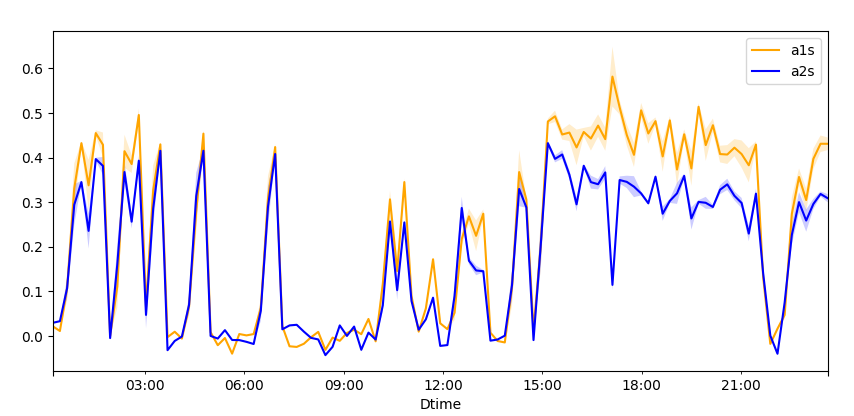
\includegraphics[width=\linewidth]{Screenshot from 2023-01-05 23-14-51.png}
    \caption{Results of the SMC2 to estimate a1, a2}
    \label{fig:smc2_results}
\end{figure}
\end{frame}

\begin{frame}{Conclusion}
We used an augmented state-space model to estimate the behavioral
parameters of seals in Alaska.
\newline
\\
However, the paper, the hypothesis and the data we worked on have several limits :

\begin{enumerate}
    \item Window : arbitrary duration of a window (26 minutes), ($a_1$,$a_2$) are not likely to be constant over a window period
    \item We don't use horizontal velocity to estimate the behavioral parameters of seals.
    \item Need recurrence in the behavioral of seals
    \item Difficult to use on other data or usecases
\end{enumerate}
\end{frame}
\begin{frame}{Appendix 1}
\begin{figure}[h]
    \centering
    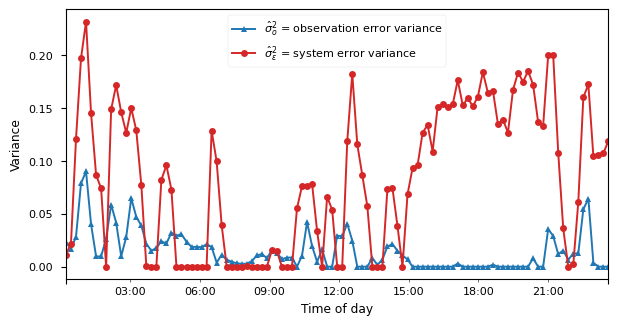
\includegraphics[width=0.8\linewidth]{var_fig.png}
    \caption{Offline estimation of the system error and observation error variances, using a quadratic regression on the ACVF for each time window.}
\end{figure}
\end{frame}

\begin{frame}{Appendix 2}
\begin{figure}[h]
    \centering
    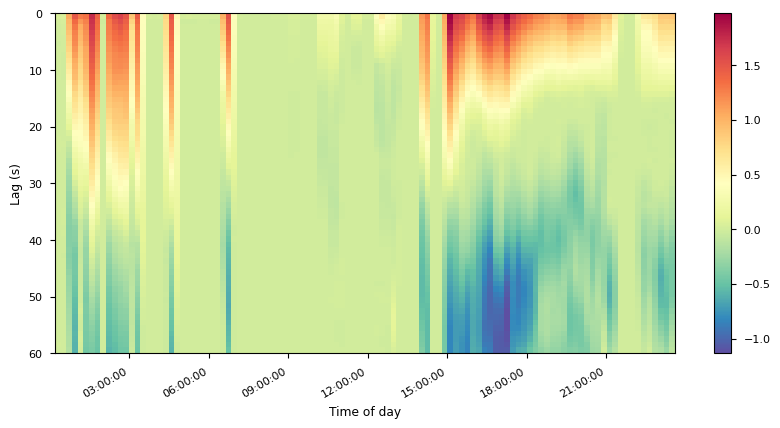
\includegraphics[width=0.8\linewidth]{acvf_fig.png}
    \caption{Estimation of the ACVF on each of the 109 time windows.}
    \label{fig:acvfs}
\end{figure}
\end{frame}

\begin{frame}{Appendix 3: Comparaison of the results}
\begin{figure}[h!]
    \centering
    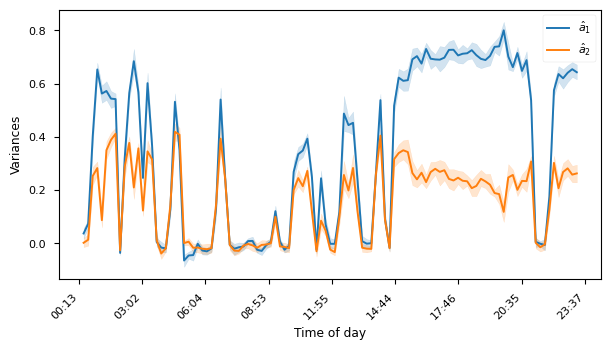
\includegraphics[scale=0.37]{a1_a2_var_0.5.png}
        \caption{Results with the method of the article}
      \label{fig:paper_results_annexes}
\end{figure}

\begin{figure}[h!]
    \centering
    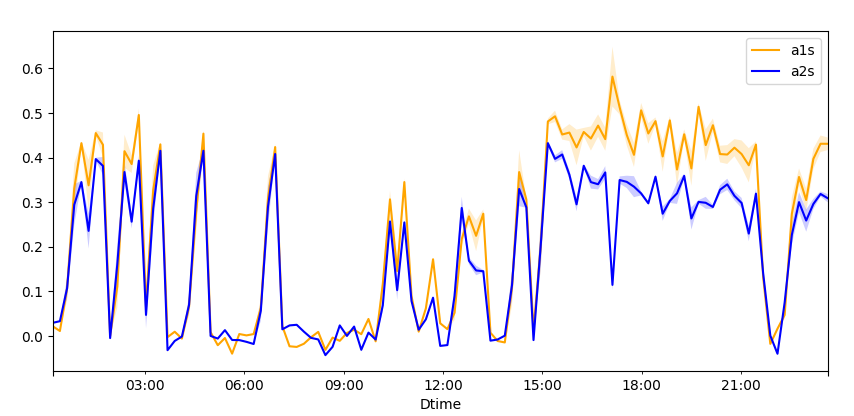
\includegraphics[scale=0.18]{Screenshot from 2023-01-05 23-14-51.png}
        \caption{Results from the $SMC^2$ model}
      \label{fig:smc2_results_annexe}
\end{figure}

\end{frame}
\begin{frame}{References}
% 1) Michael Dowd and Ruth Joy. Estimating behavioral parameters in animal movement models using a
% state-augmented particle filter. Ecology, 92(3):568–575, 2011
% \newline
% \\
% 2) Nicolas Chopin, Omiros Papaspiliopoulos, et al. An introduction to sequential Monte Carlo. Springer,
% 2020

\nocite{*}
\bibliographystyle{unsrtnat}
\addcontentsline{toc}{section}{Reference}
\bibliography{bibliography}
\end{frame}

\end{document}
